%File: formatting-instruction.tex
\documentclass[smallcondensed]{svjour3}
\usepackage{times}
\usepackage{helvet}
\usepackage{courier}
\usepackage{graphicx}
\RequirePackage{fix-cm}
\usepackage[numbers]{natbib}
\journalname{Autonomous Agents and Multi-Agent Systems}

\usepackage{amsfonts}
\usepackage{amsmath}
\usepackage{algorithmicx}
\usepackage{algpseudocode}

\usepackage{algorithm}
%\fontsize{24}{6}
%\selectfont

%TODO
%Intro
%Background
%	Agent Partitioning -- Expanded upon. I got a few "Why bother doing agent partitioning" questions.
%	Reward Shaping
%RUBI
%	Overview -- Done
%	The RUBI Algorithm -- Done
%	Reward/Utility-Based Impact -- Adds more detail about what this actually is. Was included in old paper, removed for space. -- Done
%	Simulation -- Done
%	Benefits -- Done
%Experimental Validation -- Done
%	Heterogeneous Bar Problem -- Done
%	Air Traffic Flow Management Problem -- Done
%		Agent Definition -- Done
%		Reward Structure -- Done
%		Computational Complexity -- Done
%Results
%	RUBI Performance in the Bar Problem -- Currently 2 paragraphs. Going to beef this up by adding old/RUBI partitioning comparison results from my thesis. And add more discussion on the difference in partitioning techniques. -- Done
%	RUBI Performance in the ATFMP -- Done
%		The Old Way -- Adding time/performance results from my thesis/accepted short papers
%		The RUBI Way -- Done
%		Comparison -- From my thesis. Extra results directly comparing the two in time complexity, performance, and cost-benefit analysis in these large problems.
%Discussion -- Add old/RUBI comparison cost-benefit analysis -- Done
%Conclusion -- Done
\DeclareMathOperator*{\argmin}{argmin}

\setcounter{secnumdepth}{1}  

\begin{document}

\title{Agent Partitioning with Reward/Utility-Based Impact}
\author{William Curran
\and
Adrian Agogino
\and 
Kagan Tumer
}


%Oregon State University \\
%Corvallis, Oregon \\
%curranw@onid.orst.edu \\

%NASA AMES Research Center \\
%Moffet Field, California \\
%adrian.k.agogino@nasa.gov \\

%Oregon State University \\
%Corvallis, Oregon \\
%kagan.tumer@oregonstate.edu \\
\institute{William Curran \at
              Oregon State University \\
              Corvallis, Oregon \\
              \email{curranw@onid.orst.edu}           %  \\
           \and
           Adrian Agogino \at
              NASA AMES Research Center \\
              Moffet Field, California \\
              \email{adrian.k.agogino@nasa.gov}
           \and
           Kagan Tumer \at
           Oregon State University \\
           Corvallis, Oregon \\
           \email{kagan.tumer@oregonstate.edu}
}

\date{Received: date / Accepted: date}


\maketitle


\begin{abstract}
Reinforcement learning with reward shaping is a well-established but often computationally expensive approach to solving problems involving large multiagent systems. Agent partitioning can reduce this computational complexity by treating each partition as an independent problem. Existing partitioning methods do not scale to large systems, or leverage domain-based knowledge. We introduce a novel agent partitioning approach called Reward/Utility-Based Impact (RUBI). RUBI quickly finds an effective partitioning of agents while requiring no prior domain knowledge. These partitions lead to faster simulations and when combined with reward shaping improves learning performance. We demonstrate the effectiveness of RUBI in the Air Traffic Flow Management Problem (ATFMP), where there are tens of thousands of aircraft affecting the system and no obvious similarity metric between agents. We find that partitions computed using RUBI in the ATFMP lead to a 37\% increase in learning performance when combined with reward shaping, with a 26x speed increase over non-partitioning learning approaches. Additionally, RUBI with reward shaping matches the performance of the current domain-dependent partitioning with reward shaping gold standard in the ATFMP \cite{Curran:2013:AHC:2484920.2485183} using no prior knowledge and with 10\% faster computation speed.

\end{abstract}


%\category{I.2.11}{Distributed Artificial Intelligence}{Intelligent Agents}
%\terms{
%Algorithms, 
%%Management, 
%%Measurement, 
%Documentation, 
%Performance, 
%Design, 
%Economics, 
%Reliability%, 
%Experimentation%, 
%Security, 
%Human Factors, 
%Standardization, 
%Languages, 
%Theory, 
%Legal Aspects, 
%Verification.
%}
%\keywords{Multiagent Partitioning, Multiagent Learning}
%Multiagent Systems Coordination and Collaboration Multiagent Learning





\section{Introduction}
In learning algorithms, reward design is important for keeping convergence time low while keeping performance high. In many multiagent coordination domains there is a difference between maximizing the system-level reward and maximizing a single agent's reward. If an agent always takes the locally-optimal action, it does not always maximize the system-level reward. One way to alleviate this issue is to use reward shaping. Reward shaping is a field in multiagent reinforcement learning that focuses on the design of rewards. Rather than each agent receiving a system-level reward, or a local reward, an agent can receive a reward unique to its own learned policy. Reward shaping methods have been demonstrated to improve the system-level reward in data routing \cite{tumer-wolpert_jair02}, air traffic control \cite{tumer-agogino_jaamas12}, Robocup soccer \cite{AAMAS12-agmon}, rover coordination \cite{5509316} and power plant operations \cite{Colby:2012:SFF:2343576.2343637} multiagent coordination problems. The use of reward shaping is often powerful, yet computationally expensive. In large, highly-coupled domains reward shaping can become computationally intractable. 

Modeling the reward shaping technique in relatively large domains (approximately 400 agents) removes much of this computation, but requires tens of thousands of accurate examples to compute these approximations \cite{Proper:2012:MDR:2343896.2344025}. Alternatively, partitioning agents into hierarchies \cite{tumer-holmesparker_ala12} or teams \cite{Curran:2013:AHC:2484920.2485183} speeds up computation time for larger domains (approximately 10,000-40,000 agents). Hierarchy and team approaches can use reward shaping without computing the approximation of the reward shaping technique. However, the algorithm designer must also have a fundamental understanding of how agents are coupled in order to create suitable hierarchies or teams. These approaches break down in complex or unmodeled domains.


In this paper we introduce Reward/Utility-Based Impact (RUBI). RUBI partitions agents by determining the effect of one agent's action on another agent's reward. RUBI is motivated by a simple concept: If an agent is removed from the system, how does that impact other agents? If one agent's action heavily impacts another agent's reward (positively or negatively), those agents are coupled enough to be partitioned together. It removes an agent from the system, and computes how that removal affected the other agent's local rewards. This is measured as the impact one agent has on another agent. This impact is an informative similarity metric between all agents. We then use this metric in a clustering algorithm to partition agents and reduce the complexity of the learning problem by separating the problem into smaller, independent subproblems. In contrast to many other agent partitioning approaches, this has the advantage of requiring \textit{no domain knowledge}. Since RUBI requires only a local reward, it is broadly applicable in complex domains or situations with little domain-knowledge.

We demonstrate the efficacy of RUBI in two congestion problems: a modified El Farol Bar Problem \cite{BarProblem} and the Air Traffic Flow Management Problem (ATFMP) \cite{Agogino:2009:EEM:1570256.1570258,Curran:2013:AHC:2484920.2485183,Rios}. Congestion problems are characterized by requiring a few agents to receive negative rewards in order for the rest of the agents to receive positive rewards. This can be difficult, as self-interested agents will negatively contribute to the system-level performance.

In the ATFMP the goal is to minimize both congestion and delay associated with the air traffic over the United States. There are tens of thousands of flights every day within the United States \cite{faa05}, making the search space in this problem huge. Because the airspace has many connections between airports, the congestion and associated delay can propagate throughout the system. Delays can be used to better coordinate aircraft and mitigate the propagation of congestion and the associated delay, but modeling the delay and congestion is not possible. We can apply reinforcement learning techniques to solve this problem, but this requires multiagent coordination through reward shaping. In such a large problem, reward shaping is computationally intractable \cite{Curran:2013:AHC:2484920.2485183}. We apply RUBI as a domain-independent partitioning approach to reduce the computational complexity associated with reward shaping.

%In the ATFMP, multiagent coordination with reward shaping becomes a computationally intractable task, therefore related work has applied automated agent partitioning to reduce the overhead associated with the hard constraint while computing rewards \cite{Agogino:2009:EEM:1570256.1570258,Curran:2013:AHC:2484920.2485183,Rios}. In that work, agents were only required to compute the reward relative to other agents within their partition, removing thousands of extra computations per learning step. We employ this approach, but use RUBI-based partitioning rather than the related work domain-based partitioning.

%A high level view of the approach is as follows: First, we compute partitions of agents. These partitions are treated as reward independent of each other, and therefore need to only compute rewards relative to the other agents within their partition. We will use the term \textit{reward independent} to denote one partition of agents to have no impact on the reward of other partitions. Essentially, no matter what actions one partition of agents take, it will not affect the the action choice for any agent in another partition. We then perform multiagent reinforcement learning using the difference reward. Lastly, we follow the related work approach by adding a greedy scheduler, algorithmically removing all congestion from the system at the cost to delay. Combining the multiagent reinforcement learning with reward shaping and the greedy scheduler turns this into a computationally intractable task. However, with agent partitioning, rewards can be computed many times faster with minimal performance degradation.
 
The contributions of this work are:
\begin{itemize} 
\item Generality: RUBI requires no prior knowledge of the domain. \\
\item Ease of use: RUBI removes the need to derive similarity metrics from the domain. \\
\item Performance: RUBI discovers efficient agent partitions by using the reward function to partition agents. \\
\item Speed: RUBI creates a large number of partitions without a reduction in performance. With more partitions, the reward shaping technique is faster to compute. \\
\end{itemize} 
 
The remainder of this paper is organized as follows. Section 2 describes the related work in agent partitioning, multiagent coordination, reward shaping, and the clustering. Section 3 defines reward-based impact and describes the RUBI algorithm. In Section 4 we describe our experimental validation of RUBI using multiagent coordination in both the Bar Problem and ATFMP. Experimental results are provided in Section 5 and 6, followed by  a comparison between domain-based and RUBI partitioning in Section 7. We conclude with a discussion and conclusion in Sections 8 and 9.

\section{Background}
\label{sec:BACKGROUND}

To motivate our approach, we outline previous work performed in the field of agent partitioning. We also briefly describe the reward shaping technique and clustering algorithm used throughout this work.

\subsection{Agent Partitioning}
%TODO These can be shortened. Need to have more connection between. Add in reviewers favorites and how my work is different.
Previous work in agent partitioning has focused mainly on how to divide a learning problem: by the state space, actions or goals. Jordan and Jacobs \cite{716791} developed the Hierarchical Mixtures of Experts (HME) method to partition the state space directly, such that different agents can focus on specific regions of the state space. This method works well in non-linear supervised learning tasks. However, many multiagent learning domains, such as those demonstrated in this paper, are unsupervised.

Another common solution is to partition by actions so that each agent is responsible for a small number of actions. Sun and Pearson \cite{Sun98someexperiments} divided actions into two types, and a separate agent handled each type. This approach leverages direct domain knowledge, which is not always available, and partitioning actions does not apply well in domains where all actions need to be explored.

Another approach is to partition system-level goals into smaller tasks. Dayan and Hinton \cite{Dayan93feudalreinforcement} accomplished goal partitioning through on-line task allocation, where agents are organized in a hierarchy, and high-level agents assign goals to agents lower in the hierarchy. In the work by Reddy and Tadepalli \cite{Reddy_learninggoal-decomposition}, the approach is more structured; agents learn the partitioning of the goal through externally provided examples. These approaches assume that the system-level goal can be subdivided, which is not always the case. 

Overall, current partitioning techniques work well in smaller multiagent system domains. Zhang and Lesser \cite{Zhang:2010:SCD:1838206.1838304} effectively partition 324 agents in a distributed task allocation problem. They use joint-event-driven interactions and conditional probabilities at every timestep to compute the `gain of interactions'. This additional on-line computation makes their approach computationally intractable in domains with tens of thousands of agents. Similarly, Distributed Constraint Optimization (DCOP) are well-suited for modeling multiagent coordination problems with many interactions between agents and provide theoretical performance guarantees \cite{Junges:2008:EPD:1402298.1402308,Modi:2005:AAD:1120120.1120127}. Again, these approaches have only explored relatively small domains (approx. 100 agents).

The work of Zhang and Lesser \cite{Zhang:2010:SCD:1838206.1838304} and other work in DCOPs \cite{Junges:2008:EPD:1402298.1402308,Modi:2005:AAD:1120120.1120127} have a different focus than the work presented here. The goal of those works was to effectively increase performance in their experiments. In our work we wish to provide a general technique that will scale to extremely large multiagent systems while sacrificing as little performance as possible.

%In our work, we partition agents, essentially treating each partition of agents as an independent problem. Agents from one partition could potentially affect the environment of agents in another partition, but we attempt to minimize the partition overlap. In a partitioning with complete reward independence, we essentially treat the problem as a set of smaller and easier independent problems. We will use the term \textit{reward-independent} to denote one partition of agents to have no impact on the reward of other partitions. Essentially, no matter what actions one partition of agents take, it will not affect the the action choice for any agent in another partition. 

\subsection{Difference Rewards}
\label{sec:Difference Reward}
Multiagent coordination is an important aspect of many domains, such as data routing \cite{tumer-wolpert_jair02}, air traffic control \cite{tumer-agogino_jaamas12}, Robocup soccer \cite{AAMAS12-agmon}, rover coordination \cite{5509316} and power plant operations \cite{Colby:2012:SFF:2343576.2343637}. A learning or evolutionary algorithm will often convert a computationally intractable search problem into a feasible guided search. 

In learning algorithms reward design is important for keeping convergence time low and performance high. In many multiagent coordination domains there is a difference between maximizing the system-level reward and maximizing a single agent's reward. If an agent always takes the locally optimal action, it does not always maximize the system-level reward; this is known as the Tragedy of the Commons \cite{Hardin}.

The difference reward \cite{tumer-wolpert_jair02} is evaluated such that each agent's reward is related to the individual's contribution to team performance, thereby improving the signal-to-noise ratio. This leads to learning better policies at an accelerated convergence rate. The difference reward is defined as $D_i(z) = G(z) - G(z - z_i + c_i)$, where \textit{z} is the system state, $z_i$ is the system state vector affected by agent $i$, and $c_i$ is a counterfactual replacing agent $i$. This counterfactual offsets the artificial impact of removing an agent from the system.

Each agent must calculate the difference reward for itself. For each agent, we must remove the agent from the system and recompute the global reward. In domains with tens of thousands of agents, a complex simulation, or both, this becomes computationally intractable. Removing an agent and recomputing the global reward is an $O(n^2)$ operation. With expensive simulations, the computational cost becomes intractable.  We can calculate the difference reward with respect to a small number of agents by partitioning the agents into independent groups. This means that each agent only needs to consider a small number of agents when recomputing the goal.

%In many systems it is difficult or impossible to calculate the difference reward without resimulation, which can become prohibitively costly. If resimulation is fast, or the difference reward function is easily approximated, this reward function is a powerful tool for multiagent coordination. Our work addresses this issue.
\subsection{Clustering algorithms}
Clustering algorithms group a set of objects in such a way that objects within the same group are similar to each other. The clustering operation requires either a similarity metric between objects of a feature vector for each object. We use an established clustering algorithm to create the agent partitions used in this work. The two most common and basic forms of clustering are centroid-based clustering and connectivity based clustering. Both have costs and benefits. Here we analyze those costs and benefits and explain the logic behind which algorithm we use.  

In centroid-based clustering, clusters are represented by a central vector, which may not necessarily be a member of the data set. \textit{K}-means clustering is a common centroid-based approach when the object can be represented by features \cite{Jain:2010:DCY:1755267.1755654}. In \textit{k}-means clustering, the number of clusters are fixed to k, leading to an intuitive optimization problem: find the cluster centers and assign the objects to the nearest cluster center, such that the squared distances from the cluster are minimized.

Connectivity-based clustering, also known as hierarchical clustering, is based on the idea that objects are more related to nearby objects than to objects farther away. In this method, typically an $n\times n$ similarity matrix is computed, where $n$ is the number of objects to cluster. After the similarity matrix is computed, hierarchical clustering can be performed, clustering objects one at a time based on the similarity matrix. This process repeats until one cluster remains or all clusters are independent, but is typically stopped early to get the desired number of clusters. Clustering can be stopped at any point and saved to obtain the desired number of clusters. Like k-means clustering, hierarchical clustering has been used in hundreds of applications for many years, including document clustering \cite{Zhao:2002:EHC:584792.584877} and drug design \cite{Bottegoni15072006}.

In this work, we chose connectivity-based clustering over centroid-based clustering. Centroid-based clustering uses a feature vector for every agent. In domains with tens of thousands of agents, such as the ATFMP, this imposes a very large memory requirement.
 
This work is focused around developing a similarity matrix that can be used as input to the Hierarchical Agglomerative Clustering (HAC) algorithm \cite{Manning:2008:IIR:1394399,Agglomerative}. The HAC algorithm (Algorithm 1) first computes an $N\times N$ similarity matrix $C$ and an $N$ length indicator vector $I$ where $N$ is the number of agents. Each object is initially considered to be in its own cluster, and are considered ``active'' ($I[n] = 1$). The algorithm then executes $N$-1 iterations of clustering, starting with the most similar clusters according to the similarity matrix. In each iteration two clusters, $i$ and $m$, are merged together and overwrite cluster $i$. The similarity matrix is updated based on the newly merged cluster and every other cluster, and the cluster $m$ is deactivated ($I[m] = 0$). $SIM(d_n, d_i)$ is the initial similarity between object $n$ and $i$, and is given as an argument to the algorithm. $SIM(i,m,j)$ computes the similarity between merged clusters $i$ and $m$, and another cluster $j$.

There are currently three main methods of computing cluster similarity $SIM(i,m,j)$ \cite{Manning:2008:IIR:1394399}. The first is single-link, where the updated similarity between the merged cluster and other clusters is the minimum distance $i$ or $m$ has to $j$. The second is complete-link, where the updated similarity between the merged cluster and other clusters is the maximum distance $i$ or $m$ has to $j$. The last method is average-link, where the updated similarity between the merged cluster and other clusters is the average distance $i$ and $m$ has to $j$. In this work we use the average-link similarity in order to try to obtain similar cluster sizes.

%We chose to seed the initial similarity matrix $C$ with a similarity computed by either using prior domain knowledge, such as flight plan similarity, or using RUBI, thus replacing $SIM(d_n, d_i)$.


%\begin{table}[]
%\begin{tabular}{|c|c|}
%\hline
%Name & Formula\\
%\hline
%Single-Link&$min\{d(a,b) : a \in A, b \in B\}$ \\
%\hline
%Complete-Link&$max\{d(a,b) : a \in A, b \in B\}$ \\
%\hline
%Average-Link & $\frac{1}{|A| |B|} \sum_{a \in A}\sum_{b \in B} d(a,b)$\\
%\hline
%\end{tabular}
%\caption{How $Sim$ is traditionally computed, where $d$ is a distance metric and $A$ and $B$ are the two cluster sets.}
%\label{Linking}
%\end{table}

\begin{algorithm}
  \caption{Hierarchical Agglomerative Clustering}
  \begin{algorithmic}[1]
    \Statex
    \Function{HAC}{$d_1,..., d_N$}
	  \For{$n \leftarrow 1$ to $N$} \Comment{Initialize Similarity Matrix $C$}
	    \For{$i \leftarrow 1$ to $N$}      
          \State{$C_{n,i} \leftarrow SIM(d_n, d_i)$}
          \EndFor
          \State{$I[n] \leftarrow 1$ \Comment{Activate all clusters}}
        \EndFor
        \State{$A \gets \emptyset$}
        \For{$k \leftarrow 1$ to $N-1$} \Comment{Assembles clustering as a sequence of merges}
          \State{$<i, m>$ $\leftarrow$ $argmax_{<i,m>: i \neq m \wedge I[i]=1 \wedge I[m]=1}$ $C_{i,m}$} 
          %\State{$<i, m>$ $\leftarrow$ $\underset{<i,m>: i \neq m \wedge I[i]=1 \wedge I[m]=1}{\operatorname{argmax}} C[i][m]$} 
          \State{$A \gets A \cup {<i, m>}$ 	\Comment{Store merge}}
          \For{$j \leftarrow 1$ to $N$}
            \State{$C_{i,j} \leftarrow SIM(i,m,j)$}
           	\State{$C_{j,i} \leftarrow SIM(i,m,j)$}
          \EndFor
          \State{I[\textit{m}] $\leftarrow$ 0 \Comment{Deactivate cluster $m$}}
        \EndFor
      \State \Return{$A$}
    \EndFunction
  \end{algorithmic}
\end{algorithm}

\section{RUBI}
In this section we will describe the Reward/Utility-Based Impact (RUBI) algorithm. We will first describe a general overview of RUBI and the implementation. We will then review the variety of ways to develop RUBI impact scores and simulations.

\subsection{The RUBI Algorithm}
In this work we introduce an autonomous partitioning algorithm requiring no domain knowledge, the Reward/Utility Based Impact algorithm. Domain-based partitioning analyzes the domain model and partitions agents together based on some user-defined specification. Instead, we develop an agent similarity matrix based on learning rewards received by each agent. This similarity matrix represents the impact of one agent on another. This matrix can then be used as an input to a hierarchical agglomerative clustering algorithm. Additionally, by removing all knowledge about the domain and partitioning based on reward, RUBI can be used to discover non-trivial indirect interactions encoded in a reward signal.

%RUBI uses a similar concept that motivated the difference rewards: If an agent is removed from the system, how does that affect system-level reward? 

The RUBI impact score is calculated by removing an agent from the system, and analyzing how that impacted all other agents. We assume that if one agent's action heavily impacts another agent's reward (positively or negatively), those agents are coupled enough to be partitioned together. The RUBI algorithm computes a localized reward for each agent with agent $i$ in the system, and then compares that reward to the localized reward for each agent if agent $i$ is not in the system. This partitioning algorithm is based on the central idea:
%
\begin{align}
|L_i(z) - L_i(z-z_j)| &> |L_k(z) - L_k(z-z_j)|   \Rightarrow \\
Similarity(i,j) &> Similarity(k,j) \nonumber
\end{align}
%
where $L_i(z-z_j)$ is the localized reward of agent $i$ if $j$ is not in the system, $L_k(z-z_j)$ is the localized reward of agent $k$ if $j$ is not in the system, and $L_i(z)$ and $L_k(z)$ are the localized rewards of $i$ and $k$ when all agents are in the system. This means that if the localized reward of agent $i$ changes more than the localized reward of agent $k$ when agent $j$ is taken out of the system, agent $j$ has more effect on agent $i$ than on agent $k$. This is the essential idea behind RUBI, and is encoded in RUBI (Algorithm 1) through the equation:

\begin{equation} \label{eq:RUBI Update}
C_{r,a} \leftarrow C_{r,a} + |L_a(z) - L_a(z-z_r) | \;,
\end{equation}

where $L_a(z)$ is the reward agent $a$ receives when all agents are in the system, $L_a(z-z_r)$ is the reward agent $a$ receives with agent $r$ not in the system, and $C_{r,a}$ is the cumulative impact agent $r$ has on agent $a$.

The RUBI algorithm (Algorithm 1) first initializes the impact table, an $N$ x $N$ matrix $C$, where $N$ is the number of agents within the system. It then calculates actions based on the $ACT()$ function, which is typically random action selection. RUBI then runs a simulation with all of the agents in the system and the localized reward is calculated for every agent. We then remove an agent from the system, recalculate the reward for each agent, and update the impact table, $C$. Since this is a localized reward, and the algorithm is highly parallelizable, this is a fast operation. This is a brief description of RUBI, and the following sections will explain how the impact data is computed, simulation specifics, and the $ACT()$ function.
%TODO Add inputs/outputs requirements?
\begin{algorithm} \label{alg:RUBI}
  \caption{Reward/Utility-Based Impact Algorithm}
  \begin{algorithmic}[1]
    \Statex
    \Function{RUBI}{$sim$}
      \State{$C \leftarrow 0_{N,N}$}
	  \For{$i \leftarrow 1$ to $iterations$}
	    \State{$actions \leftarrow ACT()$}	\Comment{Calculate actions for all agents}
	    \State{$sim.run(actions)$}
	    \State{$L(z) \leftarrow sim.getRewards()$} \Comment{Calculate $L$ for all agents}      
		\For{$r \leftarrow 1$ to $N$}
			\State{$sim.removeAgent(r)$}
			\State{$L(z-z_r) \leftarrow sim.getRewards()$}
			\For{$a \leftarrow 1$ to $N$}
				\State{$C_{r,a} \leftarrow C_{r,a} + |L_a(z) - L_a(z-z_r) |$}
				\EndFor
			\State{$sim.addAgent(r)$}
		\EndFor
	\EndFor      
	\State{Partitions $\leftarrow$ $HAC(C)$}  
    \EndFunction
  \end{algorithmic}
\end{algorithm}

%\subsection{Implementation}
%The impact data used to compute the similarity matrix is calculated from a localized reward or utility with respect to an agent. Typically the use of local rewards in congestion problems leads to a suboptimal solution. However, because RUBI is implemented prior to learning, we can use the local reward to identify agent similarity, and in the learning stage use a reward which will promote coordination.
%
%In this work we use reinforcement learning, but since RUBI acts outside the learning process, it can be applied to any system using a learning mechanism. RUBI uses local rewards to construct the partitions, but the developer can specifically build a localized reward for the partitioning. When computing the difference between the global reward with all agents and the global reward without a specific agent, we compute the difference reward. The difference reward represents how much an agent impacts the system, but the goal here is to find how much one agent impacts another agent.
%
%The impact table, $C$, is an accumulation of impact scores. Given enough iterations, this accumulation is informative enough to perform accurate partitioning. In this research we are interested more in the relative impact score from one agent to another, rather than what the explicit impact score is. This iterative approach requires at minimum enough iterations to evenly distribute over all actions an agent can take. Ideally each action should be sampled many times for an accurate impact estimate. 

%When we performed partitioning in the heterogeneous bar problem we use a local reward that was simply the local version of the system-level performance:

%\begin{equation}
%R = e^{-x_i(z)/c} \;,
%\end{equation}

%where $x_i(z)$ is the attendance on the night that agent $i$ went to the bar. Looking at Equation \ref{eq:BarProblem-Local} you can %see that this a local reward for the heterogeneous bar problem, and an example of using a local reward for partitioning data.


\subsection{Impact Calculation}

The impact data used to compute the similarity matrix is obtained from a localized reward or utility with respect to an agent. Learning using local rewards corresponds to greedy agents, which is undesirable in congestion problems.

In RUBI, we want to analyze the local impact one agent has on another. A traditional local reward can work, or an agent-specific reward can be specifically built for the partitioning. A high-level reward, such as the system-level reward, will not work as impact data. If we use the system-level reward as impact data, it will represent how much an agent impacts the system. The goal here is to find how much one agent impacts another agent. This makes local rewards an intuitive choice for impact measurement.

The impact table, $C$, is an accumulation of impact scores. Given enough iterations, this accumulation is informative enough to perform accurate partitioning. In this research we are interested in the relative impact score from one agent to another, rather than the value of the impact score. For a guaranteed accurate impact score, this iterative approach requires at minimum enough iterations to fully explore all actions an agent can take. In large domains, this is computationally intractable. However, in practice (Section \ref{sec:RUBI Results}) we show that this space does not need to be fully explored to have good results.

These actions are explored by the $ACT()$ function. The $ACT()$ function returns a list of agent actions to use in the RUBI simulation. The goal of $ACT()$ is to have as much of the interactive state space explored as possible, but we cannot exhaustively search the entire state space, as that would be computationally intractable. When agents take random actions, they are not driven by any motivating logic, and impact scores will be biased only toward agents who consistently impact each other. For these reasons we choose to take random actions.

%Equation \ref{eq:RUBI Update} is simply an accumulation of impact scores. Given enough iterations, this accumulation is informative enough to perform accurate partitioning. In this research we are interested more in the relative impact score from one agent to another, rather than what the explicit impact score is. This iterative approach requires at enough iterations to evenly distribute over all actions an agent can take. Ideally each action should be sampled many times for a accurate impact estimate. Future work in RUBI involves approximating the impact score of each agent by adding a learning rate and subtracting off previous impact scores per iteration. This causes $C_{r,a}$ to converge to an impact score, and analyzing this impact score may be useful in team formation or domain analysis.


\subsection{Simulation}
The simulation is also an aspect that can be varied by the developer when using RUBI. One example borrows some of the concepts from transfer learning.

The core idea of transfer learning is that experience gained in learning to perform one task can help improve learning performance in a related, but different, task. If the relationship between the first (source) task and the second (target) task is not trivial, there must be a mapping between the two tasks so that a learner can apply the older knowledge to the new task \cite{Taylor:2009:TLR:1577069.1755839}. One subset of transfer learning is transfer clustering. Given a proper mapping, clusters learned in a small simulation can be applied to a larger simulation \cite{6378284}. We can apply the same concepts developed in transfer clustering to this RUBI simulation. Any simulation can be used during partitioning, as long as there is a mapping from the RUBI simulation to the learning simulation. This approach is beneficial in domains where the simulation is costly and a mapping can be computed. 

%There are many domains, such as robotics, where random actions may cause certain failure modes, or where agents need to be in a particular area of the state space before interactions can really be analyzed. In these domains the $ACT()$ function can either sub-sample from a set of known non-failure mode actions, or be replaced with an actual learning algorithm to get the agent in a successful area of the state space before sampling. 

%\subsection{Benefits}

%One of the key strengths of RUBI is its simplicity and generality combined with computing highly informative similarity scores, leading to effective partitions, as described in Section \ref{sec:RUBI Results}. It needs no prior knowledge about the domain to perform partitioning, and simply needs a localized reward from each agent to build the similarity matrix. This makes RUBI highly generic and can be applied to any multiagent domain. It can treat the multiagent system as a black box, giving it random actions and receiving rewards. It can also discover non-trivial agent coupling. 

%Since RUBI uses a localized reward as partitioning data, any effect one agent has on another agent will be encoded in this reward. For example, if an agent $a$ is removed from the system, and agent $b$'s reward changes, it means that in some way agent $a$ affects agent $b$ in a direct or indirect way. An intuitive example of this is when two agents never directly or indirectly interact. A less intuitive, and more interesting, example is when two agents constantly interact, but do not affect each others reward. This indirect effect can be captured by RUBI and used as additional information when partitioning, leading to higher quality partitions in domains with complex interactions.

%Lastly, partitions built using RUBI are likely to be fewer in number. RUBI analyzes how the actions of one agent impact another agents reward. For example, plane $a$ and plane $b$ go through the same sectors, but are never congested. Using domain-based partitioning, two agents that go through the same sector many times would be partitioned together, so plane $a$ and plane $b$ would be partitioned together. In partitioning using RUBI, if over a few thousand trials the congestion of each plane is always 0, those planes actions never impact each others rewards, therefore they would not be partitioned together. The same is true if the congestion of each plane remains the same non-zero value, the actions do not affect the reward, therefore they are not partitioned. This leads partitioning using RUBI to find fewer partitions without loss of performance.

%Lastly, partitions built using RUBI are likely to be fewer in number. The ATFMP is a perfect example. Domain-based partitioning based on similar sectors encodes how often two aircraft can impact each other. RUBI on the other hand looks more into how the actions of one agent impact another agents reward, in this case congestion. For example, plane $a$ and plane $b$ go through the same sectors, but are never congested. Using domain-based partitioning, two agents that go through the same sector many times would be partitioned together, so plane $a$ and plane $b$ would be partitioned together. In partitioning using RUBI, if over a few thousand trials the congestion of each plane is always 0, those planes actions never impact each others rewards, therefore they would not be partitioned together. The same is true if the congestion of each plane remains the same non-zero value, the actions do not affect the reward, therefore they are not partitioned. This leads partitioning using RUBI to find fewer partitions without loss of performance.

\section{Experimental Validation}

We validate our approach in the heterogeneous bar problem and the ATFMP. The El Farol Bar Problem \cite{BarProblem} is a benchmarking domain typically used as an abstraction of a congestion domain. We use this domain to show preliminary results demonstrating the general effectiveness of RUBI before applying it to the more complex ATFMP. We then provide an overview of the ATFMP and our multiagent approach. In both experiments, agents learned using Action-Value Learning (stateless q-learning) with a zero-initialized value table \cite{Watkins92q-learning}. Action-Value Learning is a stateless approach where agents map actions to values representing the quality of that action. 

%We validate our approach in the heterogeneous bar problem and the ATFMP. The El Farol Bar Problem \cite{BarProblem} is a benchmarking domain used typically in preliminary work as an abstraction of a congestion domain. It is used in this research as preliminary work showing the general effectiveness of RUBI before applying it the more complex ATFMP. We modify this domain by introducing heterogeneous agents. We then provide an overview of one ATFMP approach developed by Curran et al. \cite{Curran:2013:AHC:2484920.2485183}, Agogino \cite{Agogino:2009:EEM:1570256.1570258} and Rios and Lohn \cite{Rios}. In both experiments, agents learned using Action-Value Learning (Stateless Q-Learning) with a zero-initialized value table. This is a stateless approach where agents map actions to values representing the quality of that action. 

In this work, we treat each partition of agents as an independent problem. This means that each agent within a partition calculates its reward only with respect to the other agents within its partition. However, agents from one partition could potentially affect the environment of agents in another partition, but we attempt to minimize the partition effect overlap. We will use the term \textit{reward-independent} to denote when one partition of agents will have no impact on the rewards of other partitions. 

\subsection{Heterogeneous Bar Problem}

The El Farol Bar Problem \cite{BarProblem} is an abstraction of congestion problems. In this problem there is a capacity $c$ which provides the most enjoyment for everyone who attends the bar on that particular night. This is a stateless one-shot problem where agents choose the night out of $k$ nights they attend the bar, and receive a reward based on their enjoyment. The bar problem local reward is a function of the attendance of that night:
%
\begin{equation} \label{eq:BarProblem-Local}
L_i = e^{\frac{-x_i(z)}{c}}
\end{equation}
%
where $x_i(z)$ is the attendance on the night agent $i$ went to the bar. The system-level reward is a simple summation of these local rewards across all agents:
%
\begin{equation} \label{eq:BarProblem-Global}
G(z) = \sum_{a \in A} e^{\frac{-x_a(z)}{c}}
\end{equation}
%
where $A$ is the set of all agents. 

From the reward, we know that if there are enough agents to be equally spread out across the bars, $n \leq ck$, this becomes a scheduling problem. This problem becomes a congestion problem when there are more than twice as many agents as the capacity for each night allows, $n > 2ck$. During every experiment, we chose agents such that $n > ck$. In this case a good group policy is for the majority of agents to attend one night, thus making agents attending that night receive a very low reward. The rest of the agents then equally distribute over the rest of the nights such that the number of agents for each other night becomes $c$, receiving the optimal reward for those nights. 

%We chose to use a modification of the El Farol Bar Problem to run initial experiments our new RUBI similarity matrix algorithm. The Bar Problem is a simple enough domain to directly check for optimal policies, and therefore we can see if the new algorithm produces partitions that can be used to converge to the optimal policy at a faster or at least equal convergence rate to the traditional partitioning technique. To do this, we must first slightly modify the Bar Problem to turn it into a partitioning and congestion problem. 

In order to test RUBI's effectiveness at partitioning in congestion problems, we modify the bar problem by introducing heterogeneous agents that can attend the bar only a subset of nights, rather than any night. The problem is still the same, but there are now $t$ types of agent. Each agent is given a random type.

This modification gives us an intuitive partitioning of agents. It would be useful for agents who can attend the same night to be partitioned together. We can then directly compare a direct learning approach that finds the near-optimal solution to the partitioning given by RUBI.

\subsection{Air Traffic Flow Management Problem}

The ATFMP addresses the congestion in the National Airspace (NAS) by controlling ground delay, en route speed or separation between aircraft. The NAS is divided into many sectors, each with a restriction on the number of aircraft that may fly through it at a given time. Additionally, each airport in the NAS has an arrival and departure capacity that cannot be exceeded. The goal of the ATFMP is to eliminate this congestion in the system while reducing the amount of delay each aircraft incurs. 

The approach we use in the ATFMP follows the same approach by Curran et al. \cite{Curran:2013:AHC:2484920.2485183}, Agogino \cite{Agogino:2009:EEM:1570256.1570258} and Rios and Lohn \cite{Rios}, who removed congestion completely from the system algorithmically through the use of a greedy scheduler. This scheduler analyzed the schedule after each agent had taken an action, and used a greedy algorithm to assign delays. This greedy approach fully removes congestion, but at the cost of additional delay. This leads to higher delay throughout the system. 

A high-level view of their approach is as follows. First, their approach computes partitions of agents using a domain-based similarity metric of sector overlap and hierarchical agglomerative clustering. They treated each partition independent of each other only when computing the reward, and therefore only computed rewards relative to the agents within a partition. They then performed multiagent reinforcement learning using the difference reward and the greedy scheduler (Figure \ref{LearningCycle}). The authors found that combining the multiagent reinforcement learning with reward shaping and the greedy scheduler turns this into a computationally intractable task. They solved this problem with domain-based agent partitioning, showing that rewards can be computed many times faster with minimal performance degradation.

\begin{figure}[]
\centering
\includegraphics[width=.75\columnwidth]{LearningCycle}
\caption{Learning cycle of agents in the Air Traffic Flow Management Problem.}
\label{LearningCycle}
\end{figure}

\subsubsection{Agent Definition}
In this paper, agents control one of 35,844 aircraft. Aircraft flight plans are from historical flight data from the FAA. Therefore, the only aspect of the environment we can change is the ground delay for each aircraft. Agents select a discrete amount of ground delay from 0 to 10 minutes in one minute increments (11 actions) at the beginning of each simulation. FAA data contains the sector location of each plane for every minute that plane was in service. Therefore, adding ground delay simply shifts a plane's flight plan by that many minutes. The greedy scheduler then checks if the flight plans cause any congestion, and further delays planes to eliminate congestion from the system.

In this formulation, agents do not have the capability to change their action based upon the system once the simulation starts, so feedback can only be given once per simulation. Because agents are given no knowledge of the environment, they have no state. This simplifies the learning problem for each agent, but complicates coordination. Agents must choose an action without prior knowledge of other agents' choices, and must learn how the environment is changing, and simultaneously what action to take.

%\subsection{Agent Learning}


%In single-agent systems, agents employing the exploration-exploitation strategies eventually come to an optimal solution \cite{Sutton98reinforcementlearning}. In multiagent systems the exploration of other agents become an issue. When an agent takes a greedy action, other agents can learn how that affected the environment, and modify their own greedy action. When an agent takes an exploratory action rather than a greedy action, other agents modify their greedy action based on how the environment changed with the exploratory actions. Agents learn to compensate for the exploratory actions in the system, so when exploration removed after some learning performance often decreases. This behavior is caused by exploratory noise \cite{holmes-aamas}.

%With so many agents in this system, exploratory noise causes a large problem. In the beginning of learning, having a large exploration is beneficial for the system. With 10\% of the agents taking random actions, we can find a good area of the reward space to explore. But near the end of learning, with most agents almost converged to a nearly optimal solution, 10\% of agents are taking random actions, causing over 3,500 agents to introduce noise into the learning of all other agents. To circumvent this problem, we need to have more agents performing greedy action selection as during each consecutive learning step. Therefore, $\epsilon$ would need to be lowered throughout learning to accomplish this. We approached this problem by reducing $\epsilon$ every n time steps by a constant amount (more sophisticated techniques such as the Boltzmann equation could be used, but only simple $\epsilon$ reduction was needed). The following equation was applied to $\epsilon$ at every time step:

%\begin{equation}
%\epsilon = \epsilon * c^{t * \Theta(t \mod n)}\;,
%\end{equation}
 
%where c is a constant value (typically .99), $t$ is the current time step and $\Theta(t \mod n)$ is a step function that equals 1 when $t \mod n$ is 0 and 0 otherwise, and $n$ is a value that varied depending on the number of learning steps. With more learning steps $n$ was higher, and in experiments with fewer learning steps $n$ was lower.

\subsubsection{Reward Structures}

In this section we first develop the system-level reward. This reward represents how well the system as a whole is performing. We then develop the difference reward from the system-level reward. The difference reward represents how much a particular agent contributes to the system-level reward. Agents should be rewarded with the difference reward, and system performance should be measured as the system-level reward. 

The system-level reward, $G(z)$, in the ATFMP is defined as:
%
\begin{equation} \label{eq:Global}
G(z) = -(C(z) + \delta(z))\;,
\end{equation}
where the total congestion penalty, $C(z)$, is the sum of differences between sector capacity and the current sector congestion and the total delay, $\delta(z)$, is the sum of delays over all aircraft.

%where $C(z)$ is the total congestion penalty, and $\delta(z)$ is the cumulative system delay:
%\begin{equation} \label{eq:Cumilative Delay}
%\delta(z) = \displaystyle\sum\limits_{a \in A} (\delta_{g,a}(z) + \delta_{s,a}(z))\;,
%\end{equation}
%where $\delta_{g,a}(z)$ is the ground delay the aircraft incurred and $\delta_{s,a}(z)$ is the scheduler delay the aircraft incurred. 

Agogino and Rios \cite{Agogino:2009:EEM:1570256.1570258} originally employed a greedy scheduler to algorithmically remove congestion from the system, while simultaneously using learning to minimize delay. We follow this approach, and therefore our system-level reward is simply the delay in the system:

\begin{equation}
G(z) = -\delta(z)
\end{equation}

With so many agents, tens of thousands of actions simultaneously impact the system, causing the system-level reward to become noisy with the actions of other agents. A difference reward function reduces much of this noise, and is easily derived from the system-level reward:
%
\begin{equation}
D_i(z) = - \delta(z) + \delta(z-z_i + c_i)\;,
\end{equation}
%
where \textit{$\delta(z-z_i + c_i)$} is the cumulative delay of all agents with agent $i$ replaced with counterfactual \textit{$c_i$}.

When using RUBI in the ATFMP we developed a partitioning reward by simplifying the simulation and using congestion information. At a high level we want to encapsulate how one agent affects another in the reward. We removed the greedy scheduler and used the congestion as information for the similarity data:
%
\begin{equation} \label{eq:RUBI ATFMP-L}
R = -(C(z))\;.
\end{equation}
%
This is an example of transfer clustering. Our rewards and simulations are different during partitioning than during learning.

\subsubsection{Computational Complexity}
\label{sec:Complexity}
When performing reinforcement learning with the difference reward, you must remove an agent and recompute the system-level reward. This computation occurs once for each agent. In the ATFMP, the system-level reward is the summation of delays, an $O(n)$ routine. Therefore, each learning iteration is on the order of $O(n * O(removeAgent(a)) + n^2)$, where $n$ is the number of agents. In the ATFMP each $removeAgent(a)$ call must call the greedy scheduler, an $O(n)$ algorithm, leaving the time complexity of the learning system to remain $O(n^2)$. The cost of removing an agent dominates the cost of computing the agent reward in domains where the complexity of removing an agent becomes larger than linear time. In those cases the agent partitioning becomes more useful.

When using agent partitioning, this time complexity can be drastically reduced. When computing time complexity, $n^2$, can be replaced with the number of agents per partition $p_n$ squared multiplied by the number of partitions, $p$:
%
\begin{equation}
O(n^2) = O(p_n^2 * p)
\end{equation}
%
With many agents we see a significant speedup. If we have 10,000 agents in the system, and convert that to 100 partitions of 100 agents we get $10^6$ iterations as opposed to $10^8$, two magnitudes lower. Additionally, the more partitionable the domain, the better the speed up performance. If a domain is highly partitionable, then $p$ becomes larger and $p_n$ becomes smaller, meaning fewer agents per partition. This lowers time complexity by lowering the faster-growing term. This becomes extremely important when $removeAgent(a)$ involves a high time complexity operation. Also, keep in mind this is a growth rate complexity analysis. In actuality, the speed up is much higher. For example, in the ATFMP the greedy scheduler only has to reschedule the number of agents within each partition, rather than all agents.

%We used a non-zero counterfactual for two reasons. One, when an aircraft is removed from the system, the reward given to the agents is artificially increased. Furthermore, the aircraft are less likely to cause conflicts due to the easier scheduling problem. Two, we used a counterfactual where the agent does not delay at all, meaning that if not delaying produces a higher reward than delaying, this should be found quickly. We also take advantage of the fact that most airplanes do not need to be delayed. If the counterfactual is equal to the agent removed, the difference reward becomes zero and does not need to be calculated, thus speeding up reward calculations.

\section{Optimization with Domain-Based Partitioning}
\label{sec:Domain-Based}

We first performed optimization with domain-based partitioning. The results are compared with RUBI partitioning in Section \ref{sec:Comparison}. In both approaches, we applied Hierarchical Agglomerative Clustering (HAC) to partition similar agents together. For domain-based partitioning, the similarity of each agent was computed as the number of similar sectors they had within their flight plan. In this way agents that impact each other are partitioned together. HAC was then applied using the average-linking metric and was saved at every iteration to obtain a varying size of partitions for comparison purposes. Since our distance metric was a count of similar sectors, choosing the average-linking clustering metric was natural, as we are interested in how similar clusters are on average, rather than based on least or most similar members. This clustering was executed during the pre-processing of the flight plan data. Partitioning reduced the number of aircraft into a more manageable size for learning, from 35,844 to on the order of hundreds or thousands, depending on how many partitions we used. All results reported are from 25 statistical runs.
 
\subsection{Domain-Based Partitioning Performance in the ATFMP}

By adding the greedy scheduler we were able to eliminate congestion by sacrificing delay. Some aircraft in normally highly-congested areas are forced to delay many hours, while most aircraft don't need to delay at all. Although high, this delay is required to guarantee a safe environment for all aircraft. 

Although the greedy scheduler is suboptimal, it performs well in this domain without the use of learning. Most planes do not need to be delayed, and the ones that do can simply be delayed until no congestion occurs. This solution does not take into account any interactions between aircraft, and cannot perform the coordination required to reduce delay even further. Our approach finds a better solution by finding these subtle coordination situations and taking advantage of them.  

As mentioned earlier, the greedy scheduler computes a good, but sub-optimal scheduling policy. This leads us to use the greedy scheduling policy as a good place to start searching. Initializing each agent to choose zero delay reduces the overall amount of computation time needed to compute the difference reward by giving the agents a good policy from the start. Agents can then explore other actions with a frequency based on the exploration rate and can discover potentially better actions.
  
Figure \ref{ClusterRewardsGreedyG} shows our domain-based partitioning in the ATFMP with agents learning using the system-level reward. Although using partitions are an improvement, using the system-level reward still does not minimize delay more than the simple greedy solution. This reward function does not give the agents an accurate enough learning signal to discover the subtle coordination improvements, and additionally takes a very long time to converge to a suboptimal solution. 

\begin{figure}[]
\centering
\includegraphics[width=.75\columnwidth]{ClusterRewardsGreedyG}
\caption{The highest level of partitioning for the system-level reward (G) is displayed here and compared with a single partition and the greedy scheduler. The learned policies initially perform similarly to the greedy scheduler because the policy for each agent is initialized with zero delay actions. The system-level reward performed worse with fewer partitions, but still better than a single partition. Even though partitioning performed better than a single partition, the system-level reward could not come close to beating the greedy scheduler. Using this learning approach, the system-level reward performance could never become better than the greedy scheduler.}
\label{ClusterRewardsGreedyG}
\end{figure}

The difference reward is able to communicate to the agents a reward that is more representative of their contribution to team performance. This reward reduces the signal-to-noise ratio and leads to better system-level performance. 

Figure \ref{ClusterRewardsGreedyG} shows the best-performing simulation using the system-level reward involved the highest number of partitions. Alternatively, in Figure \ref{ATFMPOldDvsGreedy} the best performing simulation with the difference reward used the lowest number of partitions. As the number of agents per partition increased, more agents affect the reward. The system-level reward has no way for an agent to filter out the noise of other agents, and therefore benefits more from having fewer agents in each partition. The difference reward, on the other hand, removes the noise from the system-level reward and agents can therefore coordinate more easily in larger partitions.

\begin{figure}
\centering
\includegraphics[width=.75\columnwidth]{ATFMPOldDvsGreedy}
\caption{A closer look at the difference reward performance using the smaller number of partitions shows a 37\% improvement over the greedy scheduling solution.}
\label{ATFMPOldDvsGreedy}
\end{figure}

Although it would result in the best performance, using the difference reward with the greedy scheduler is an impossible task. With around 35,000 aircraft in the system, one reward step takes 3 hours of execution time (2.4 GHz quad-core computer) due to the rescheduling needed at every difference calculation. Agent partitions allowed us to greatly decrease simulation time, because only agents within a partition need to be rescheduled during the difference calculation. Figure \ref{ATFMPOldDvsGreedy} shows the magnitude of performance gain when using the difference reward and partitioning. Table \ref{ATFMPOldTable} shows that the speedup of using different partition sizes is significant, but has a high cost to performance. Since partitions had some overlap, actions in one partition may affect the agents in another partition, meaning that the higher the number of partitions the less information the agents receive about the environment. A smaller number of partitions ends up leading to better overall performance at the cost of computation time.

\subsection{Partition Comparisons with Domain-Based Partitioning}
Computation speed and performance of partitions were negatively correlated. As the number of partitions reduced, the greedy scheduler was required to schedule more aircraft per difference calculation. This greatly increased the amount of time per learning step. Additionally, with a smaller number of partitions, planes that slightly affected each other were partitioned together. This led to more efficient learning since an agent's reward encompassed the effects of at most all of the other agents that impact it. 

%This speed and performance correlation also occurs within the same partition. As the delay decreases, more agents switch from selecting zero delay to selecting a more cooperative action that allowed better scheduling. This means that the agent no longer equals the counterfactual, and the difference reward calculation cannot be skipped. Table \ref{ATFMPOldTable} shows this in more detail. This table compares the amount of time taken per simulation step to the final performance.

\begin{table}
\begin{tabular}{|l|c|c|}
\hline
Number of Partitions & Average Time/Learning Step (s) & Converged Performance $G(z)$\\
&  & Delay (\textit{min}) \\
\hline
Greedy & * & 153502 \\
\hline
3 & 483.76 & 97688 \\
\hline
50 & 42.11 & 124056 \\
\hline
100 & 22.43 & 128021 \\
\hline
150 & 20.91 & 121074 \\
\hline
200 & 17.37 & 145844\\
\hline
250 & 14.27 & 152402 \\
\hline
\end{tabular}
\caption{With the greater number of partitions, the learning performance decreases and speed increases. Note that the outlier is a artifact of the greedy scheduler discussed in this section.}
\label{ATFMPOldTable}
\end{table}

The greedy scheduler includes bias when comparing experimental runs. The greedy scheduler schedules planes in order, such that the delay is a function of the aircraft ordering. During partitioning, the aircraft ordering changes for different partition sizes. Therefore, the initial greedy scheduling solution causes some bias in the trends we show here. For example, the greedy scheduler can initialize a particular partition to a better initial policy than a different partition size, causing bias in the comparisons. This greedy scheduling bias isn't large enough to impact the overall trend.

The agent partitioning allows applications to become situation dependent. If the system designer needs results very quickly, a larger number of partitions could be used. This approach with more partitions can still find a policy better than the greedy scheduler. On the other hand if run time is plentiful, the smaller number of partitions results in a policy 37\% better than the greedy scheduler, and still 23x faster per learning step than non-partitioning based approaches. The same trends found in this section are expected in the partitioning using RUBI.


\section{Optimization with RUBI} \label{sec:RUBI Results}
During preliminary analysis, RUBI works as expected in simple congestion problems, such as the El Farol Bar Problem \cite{BarProblem}. When we apply RUBI during partitioning in the ATFMP, execution time decreases and the generality of RUBI is demonstrated. The removal of domain knowledge allows the same RUBI algorithm to be used in simple problems as well as the ATFMP with no effort and without any need to develop a similarity metric.

%Partitions developed using RUBI uses similarity metrics that encapsulated the agent coupling. In this section we will first show how RUBI partitioning works well in the ATFMP, and analyze the cost/benefit of varying the number of partitions. We will then compare RUBI-based partitioning to domain-based partitioning and see that RUBI develops better quality partitions as well as partitions that lead to faster simulation times.

\subsection{RUBI Performance in the Bar Problem}
%In our formulation of the heterogeneous bar problem each agent is placed on a team of other agents who go on the same subsets of days. In this benchmarking test we are under the assumption that we do not have any access to domain knowledge, and we cannot make the simplifying assumption that agents on the same night receive the same reward. This is to further generalize the bar problem and show that partitioning with RUBI is both general, and effective in domains where domain knowledge cannot be used. 

In our formulation of the heterogeneous bar problem each agent is placed on a team of other agents who go on the same subsets of days. We used 10 nights, 1000 agents, and 10 different types of agents during experimental runs. Each type of agent is associated with a randomly-generated set of three nights that the agents of that type can visit the bar, and each agent was randomly assigned a type. %Although this formulation of the bar problem makes it easier to directly find a solution, it shows RUBI can find a partitioning of agents with no domain knowledge, and have generalized results that can give some insight to the performance of RUBI in the ATFMP. 

When partitioning agents with RUBI in the heterogeneous bar problem agents took random actions, and the localized reward was simply the local reward used traditionally (Equation \ref{eq:BarProblem-Local}). In this experiment, partitions had some overlap, as it is unlikely that there is a type of agent completely reward independent from all other types. This causes performance to degrade when using partitioning. Figure \ref{BarProblemNewPartitions} shows that this degradation is minimal with fewer partitions, and increases as more partitions are added, and additionally shows the computational speed-up involved when having many smaller partitions. This emphasizes the fact that partitioning without reward independent partitions increases speed at the cost of performance.

\begin{figure}
\centering
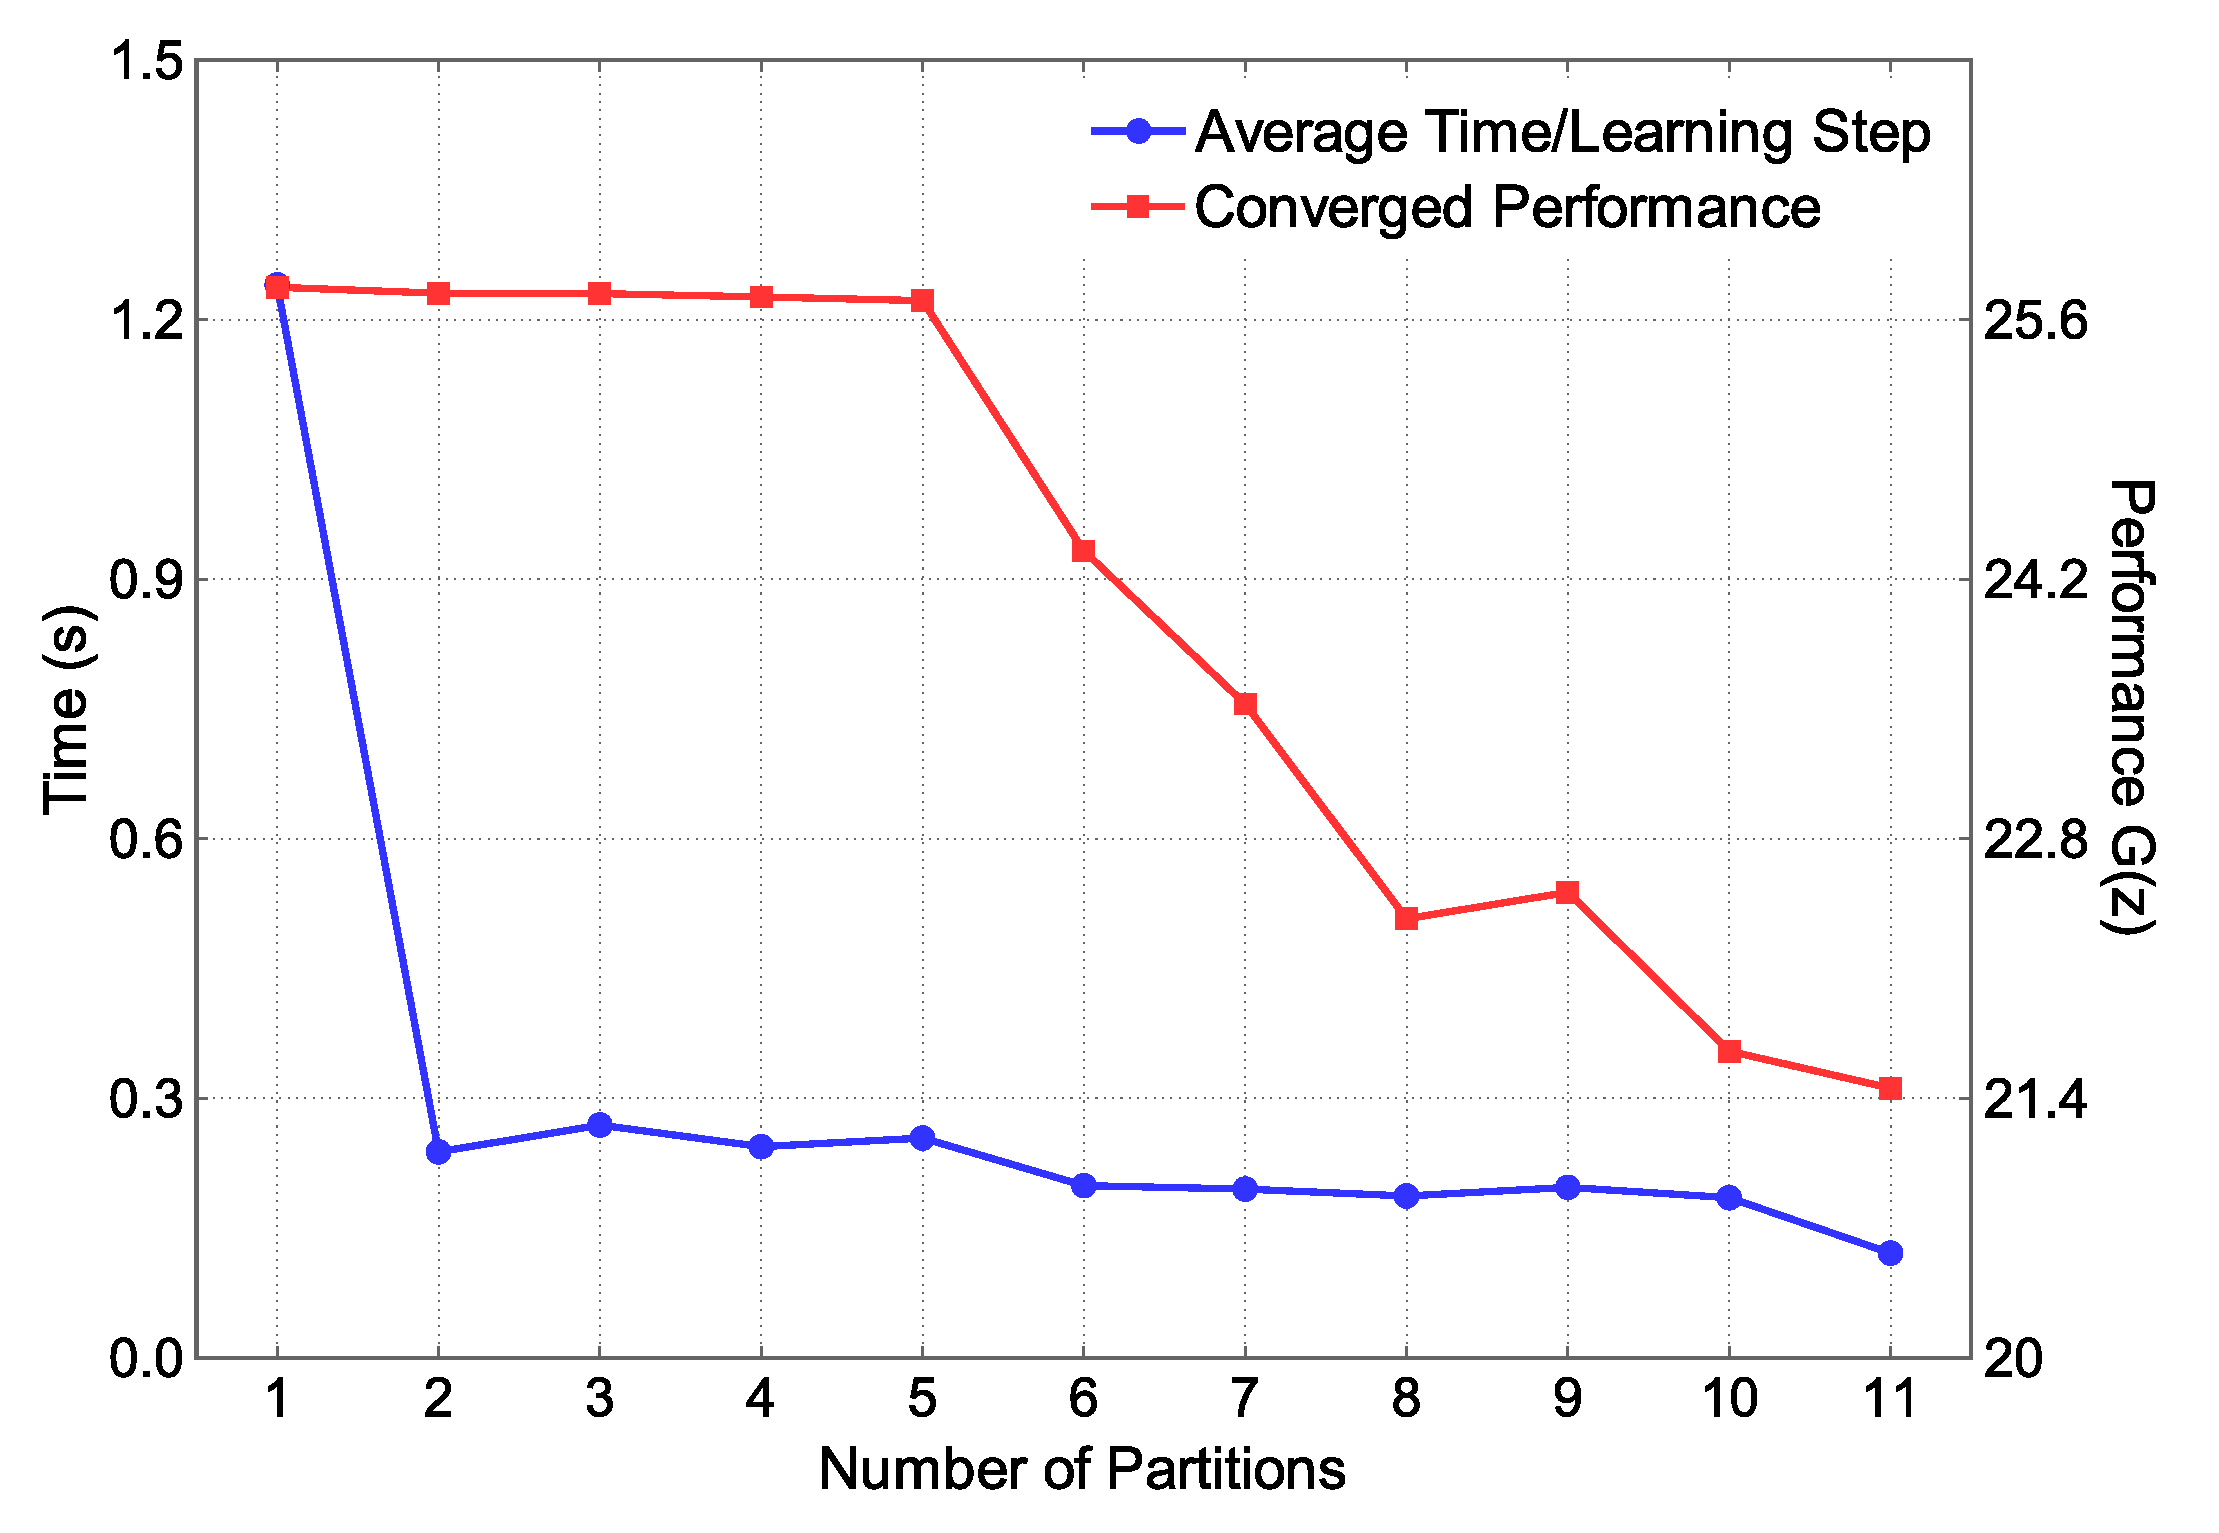
\includegraphics[width=.75\columnwidth]{BarProblemComparisonNoScale}
\caption{As the number of partitions decrease, the agents receive more information about the environment, leading to better performance at the cost of speed. }
\label{BarProblemNewPartitions}
\end{figure}

\subsection{RUBI Performance in the ATFMP}

When partitioning agents using RUBI in the ATFMP agents took random actions, the greedy scheduler was not used, and the localized reward for each agent involved only congestion (Equation \ref{eq:RUBI ATFMP-L}). Using RUBI, agents were partitioned together based on whether their actions cause other agents to experience congestion. 

Partitioning with RUBI combined with using the difference reward outperformed the greedy scheduler. Figure \ref{ATFMPComparisonNoScale} shows a variety of partitions outperforming the greedy scheduler. During analysis, we found that the final performance of the ATFMP using RUBI-based partitioning was similar to domain-based partitioning performance. This is because at a converged partitioning, all agents are considered reward-independent. The key benefit of RUBI-based partitioning was that a reward-independent partition involved 61 partitions (Figure \ref{ATFMPComparisonNoScale}), but in domain-based partitioning the smallest was 3 (Figure \ref{ATFMPOldDvsGreedy}). This leads to faster processing time at no cost to performance.

\begin{figure}
\centering
\includegraphics[width=.75\columnwidth]{ATFMPComparisonNoScale}
\caption{Like in Figure \ref{BarProblemNewPartitions}, as the number of partitions decreases, the agents receive more information about the environment. This leads to better performance at the cost of speed. The HAC algorithm converged to 61 independent partitions.}
\label{ATFMPComparisonNoScale}
\end{figure}

When partitioning in a multiagent system, unless partitions are reward-independent, there is a trade-off between faster simulation time/reward calculation and performance. When partitioning with RUBI, with the slowest simulation there is a 37\% increase in performance over the greedy scheduler, with a 26x speed up over non-partitioning approaches, and with a larger number of partitions we obtained a 1000x speed increase with a 20\% increase in performance (Figure \ref{ATFMPComparisonNoScale}).

In addition, the partitioning using RUBI converged to a reward-independent partitioning that included many more partitions than domain-based partitioning. In a reward-independent partitioning, more partitions reduce the computation while incurring no loss of performance. The reward-independent domain-based partitioning included 3 partitions, while partitioning with RUBI yielded 61 partitions. This is due to using reward-based impact as a similarity metric. The actions of two agents may greatly affect each other during simulation, but their reward-based impact on each other might still be zero. For example, if two agents go through the same sectors, but neither agent causes another agent more or less congestion, then the difference in local reward will be zero, even though those aircraft affect each other. This leads to more partitions and faster simulations. %This is an example of RUBI finding a non-trivial partitioning.

%In the ATFMP, this partitioning benefit speeds up computation by magnitudes, but how much performance are we losing, and at what point is the partitioning costing too much performance for the benefit of faster computation? Figure \ref{NewPartitionComparisons} compares average computation time, final performance and self-similarity of each partition. The average computation time per learning step for each partition size remains static, and then exponentially increases once the self-similarity becomes large. This is the cost of each partition. There is also has a sharp increase in final performance as the self-similarity increases. This is the benefit of each partition. Both of these performance metrics are correlated greatly with the self-similarity metric.

%Graph \ref{ATFMPCostBenNew} shows the benefit/cost ratio for each partition. At 100 partitions the benefit begins greatly outweighing the cost. If performance is important, 50 partitions reaches 80\% of the max performance, at only a 20\% speed up, but if a faster result is more important, 70\% of max performance can be reached with 90\% faster learning steps.

%\begin{figure}
%\centering
%\includegraphics[width=1.0\columnwidth]{NewPartitionComparisons}
%\caption{As the self-similarity increases, final performance and time taken per learning step increases. Note that final performance %is a 6th degree polynomial trend line with $R^2 = .95$, and all values are scaled between 0 and 1 for comparison purposes.}
%\label{NewPartitionComparisons}
%\end{figure}

%\begin{figure}
%\centering
%\includegraphics[width=1.0\columnwidth]{ATFMPCostBenNew}
%\caption{}
%\label{ATFMPCostBenNew}
%\end{figure}

%\subsection{Comparison Between RUBI and Domain-Based Partitioning}

%The comparisons made in this section are made with respect to the similarity metric chosen by Curran et al. \cite{Curran:2013:AHC:2484920.2485183}, Agogino \cite{Agogino:2009:EEM:1570256.1570258} and Rios and Lohn \cite{Rios}, the number of overlapping sectors between aircraft flight plans. RUBI-based partitioning benefits from ease-of-use and generality. With RUBI a very well performing partitioning can be computed with little or no effort.

%To understand how much overlap partitions had with each other, we analyzed the similarity each partition had with itself, and the average similarity each partition had with other partitions. Similarity was defined as the similarity metric used in domain-based partitioning, the number of similar sectors between agents.

%In this section, we find the number of sectors that are similar between planes in a partition (self-similarity). We then find the the average number of sectors each plane in one partition has in common with each plane in another partition, and average all of these together to obtain a other-similarity metric. When graphing these metrics we take the percentage of self-similarity to other-similarity, and vice-versa. In a purely reward-independent partition, the other-similarity is 0, and the self-similarity is 1. As the amount of self-similarity increases though, the computation time increases exponentially, reducing the computational benefits of partitioning.

%The key difficulty in performing partitioning in the ATFMP, where almost every agent is coupled, is to partition agents in such a way that the similarities between partitions are as small as possible, while still preserving the computational benefits of partitioning. For this reason, we need to analyze both the performance of a variety of partition sizes, as well as the cost associated with the partition sizes.

%Partitioning with RUBI developed better similarity scores than domain-based partitioning (Figure \ref{Self-SimOldvsSelf-SimNew}). By partitioning using congestion, the similarity metric was able to represent both similar sectors as well as sector congestion. Consider the case where two aircraft have the same flight plan, excluding their arrival and departure location. These aircraft would be partitioned together when using only similar sector domain knowledge. With RUBI, those aircraft would be partitioned together with aircraft that cause them congestion. By partitioning using the impact one agent had on another agents reward, we are able to formulate higher quality partitions, without the overhead of developing similarity metrics or learning domain knowledge.

%\begin{figure}
%\centering
%\includegraphics[width=.75\columnwidth]{Self-SimOldvsSelf-SimNew}
%\caption{Partitions formed with RUBI had higher self-similarity than using domain-based partitioning. This leads to higher quality %learning with respect to each partition.}
%\label{Self-SimOldvsSelf-SimNew}
%\end{figure}

%In addition to higher self-similarity, the partitioning using RUBI converged to a reward-independent partitioning that included many more partitions than domain-based partitioning. In a reward-independent partitioning, more partitions reduce the computation while incurring no loss of performance. The reward-independent domain-based partition included 3 partitions, while partitioning with RUBI included 61 partitions. This is due to using reward-based impact as a similarity metric. The actions of two agents may greatly affect each other during simulation, but their reward-based impact on each other might still be zero. %For example, if two agents go through the same sectors, but neither agent causes another agent more or less congestion, then the difference in local reward will be zero, even though those aircraft affect each other. This leads to more partitions, and faster simulations. This is an example of RUBI finding a non-trivial partitioning.

%When comparing final performance, a direct comparison of performance is not adequate. This is because partitions are not evenly distributed, which causes extremely large bias when comparing final performance to number of partitions. To show this in detail, we directly compared performance. We saw that with a larger number of partitions domain-based partitioning initially out performs RUBI, but RUBI began out performing domain-based partitioning with a smaller number of partitions. 

%In looking deeper into the reasoning behind this, we realize that partitions are not evenly distributed. Initially, domain-based partitioning have very large partitions compared to RUBI partitioning. This is due to the accumulation of similar sectors in domain-based partitioning. In domain-based partitioning, all of the planes with high overlap are initially merged together, giving domain-based partitioning initially larger partitions. Since this is a highly-coupled domain, this also leads to one partition becoming much larger than others. This is not seen in the self-similarity due to self-similarity being an average of all self-similarities. Basically, domain-based partitioning in this domain results in one partition having very high self-similarity, while other partitions get ignored. Although performance is initially better in domain-based partitioning, it is at 800+ partitions, meaning that the performance at this level of partitioning is already low for both partitioning approaches, and is therefore less useful.

%RUBI, which partitions based on the reward of congestion and delay, initially merged together partitions whose reward highly impacted each other, which creates more evenly distributed partitions, leading to a better overall similarity, but initially worse performance. With a smaller number of partitions, RUBI-based partitions end up becoming larger on average. This in turn led to a bias for RUBI partitioning. Note that when all partitions are reward independent, RUBI partitioning included a much smaller average size, and many more partitions.

%This results in us comparing final performance to the average size of the top 5\% of partitions. This gives a comparison of how well a partitioning performs with respect to the size of it's partitions, rather than the number. Figure \ref{ATFMPPerformancevsAvgSize} shows that initially in domain-based partitioning, learning performance does not increase with respect to the average size of the partitions. RUBI on the other hand creates a partitioning with constantly increasing performance. One key point of this figure is that RUBI-based partitioning developed a better partitioning with every additional partition merge. This is because RUBI uses rewards to develop an impact score, so when two partitions are merged together it is guaranteed that performance will increase. Domain-based partitioning on the other hand had a steady performance until a certain point, and then performance increased dramatically. Note how many points are sampled for domain-based partitioning in Figure \ref{ATFMPPerformancevsAvgSize} for the smaller sized partitions.

%\begin{figure}
%\centering
%\includegraphics[width=1.0\columnwidth]{OldvsNewAvgSize}
%\caption{Initially, domain-based partitioning has a larger average size of partitions, leading to a higher initial performance. Note %that when all partitions are reward independent, domain-based partitioning had only a few number of very large partitions. RUBI %partitioning on the other hand included a much smaller average size, and many more partitions. }
%\label{OldvsNewAvgSize}
%\end{figure}

%\begin{figure}
%\centering
%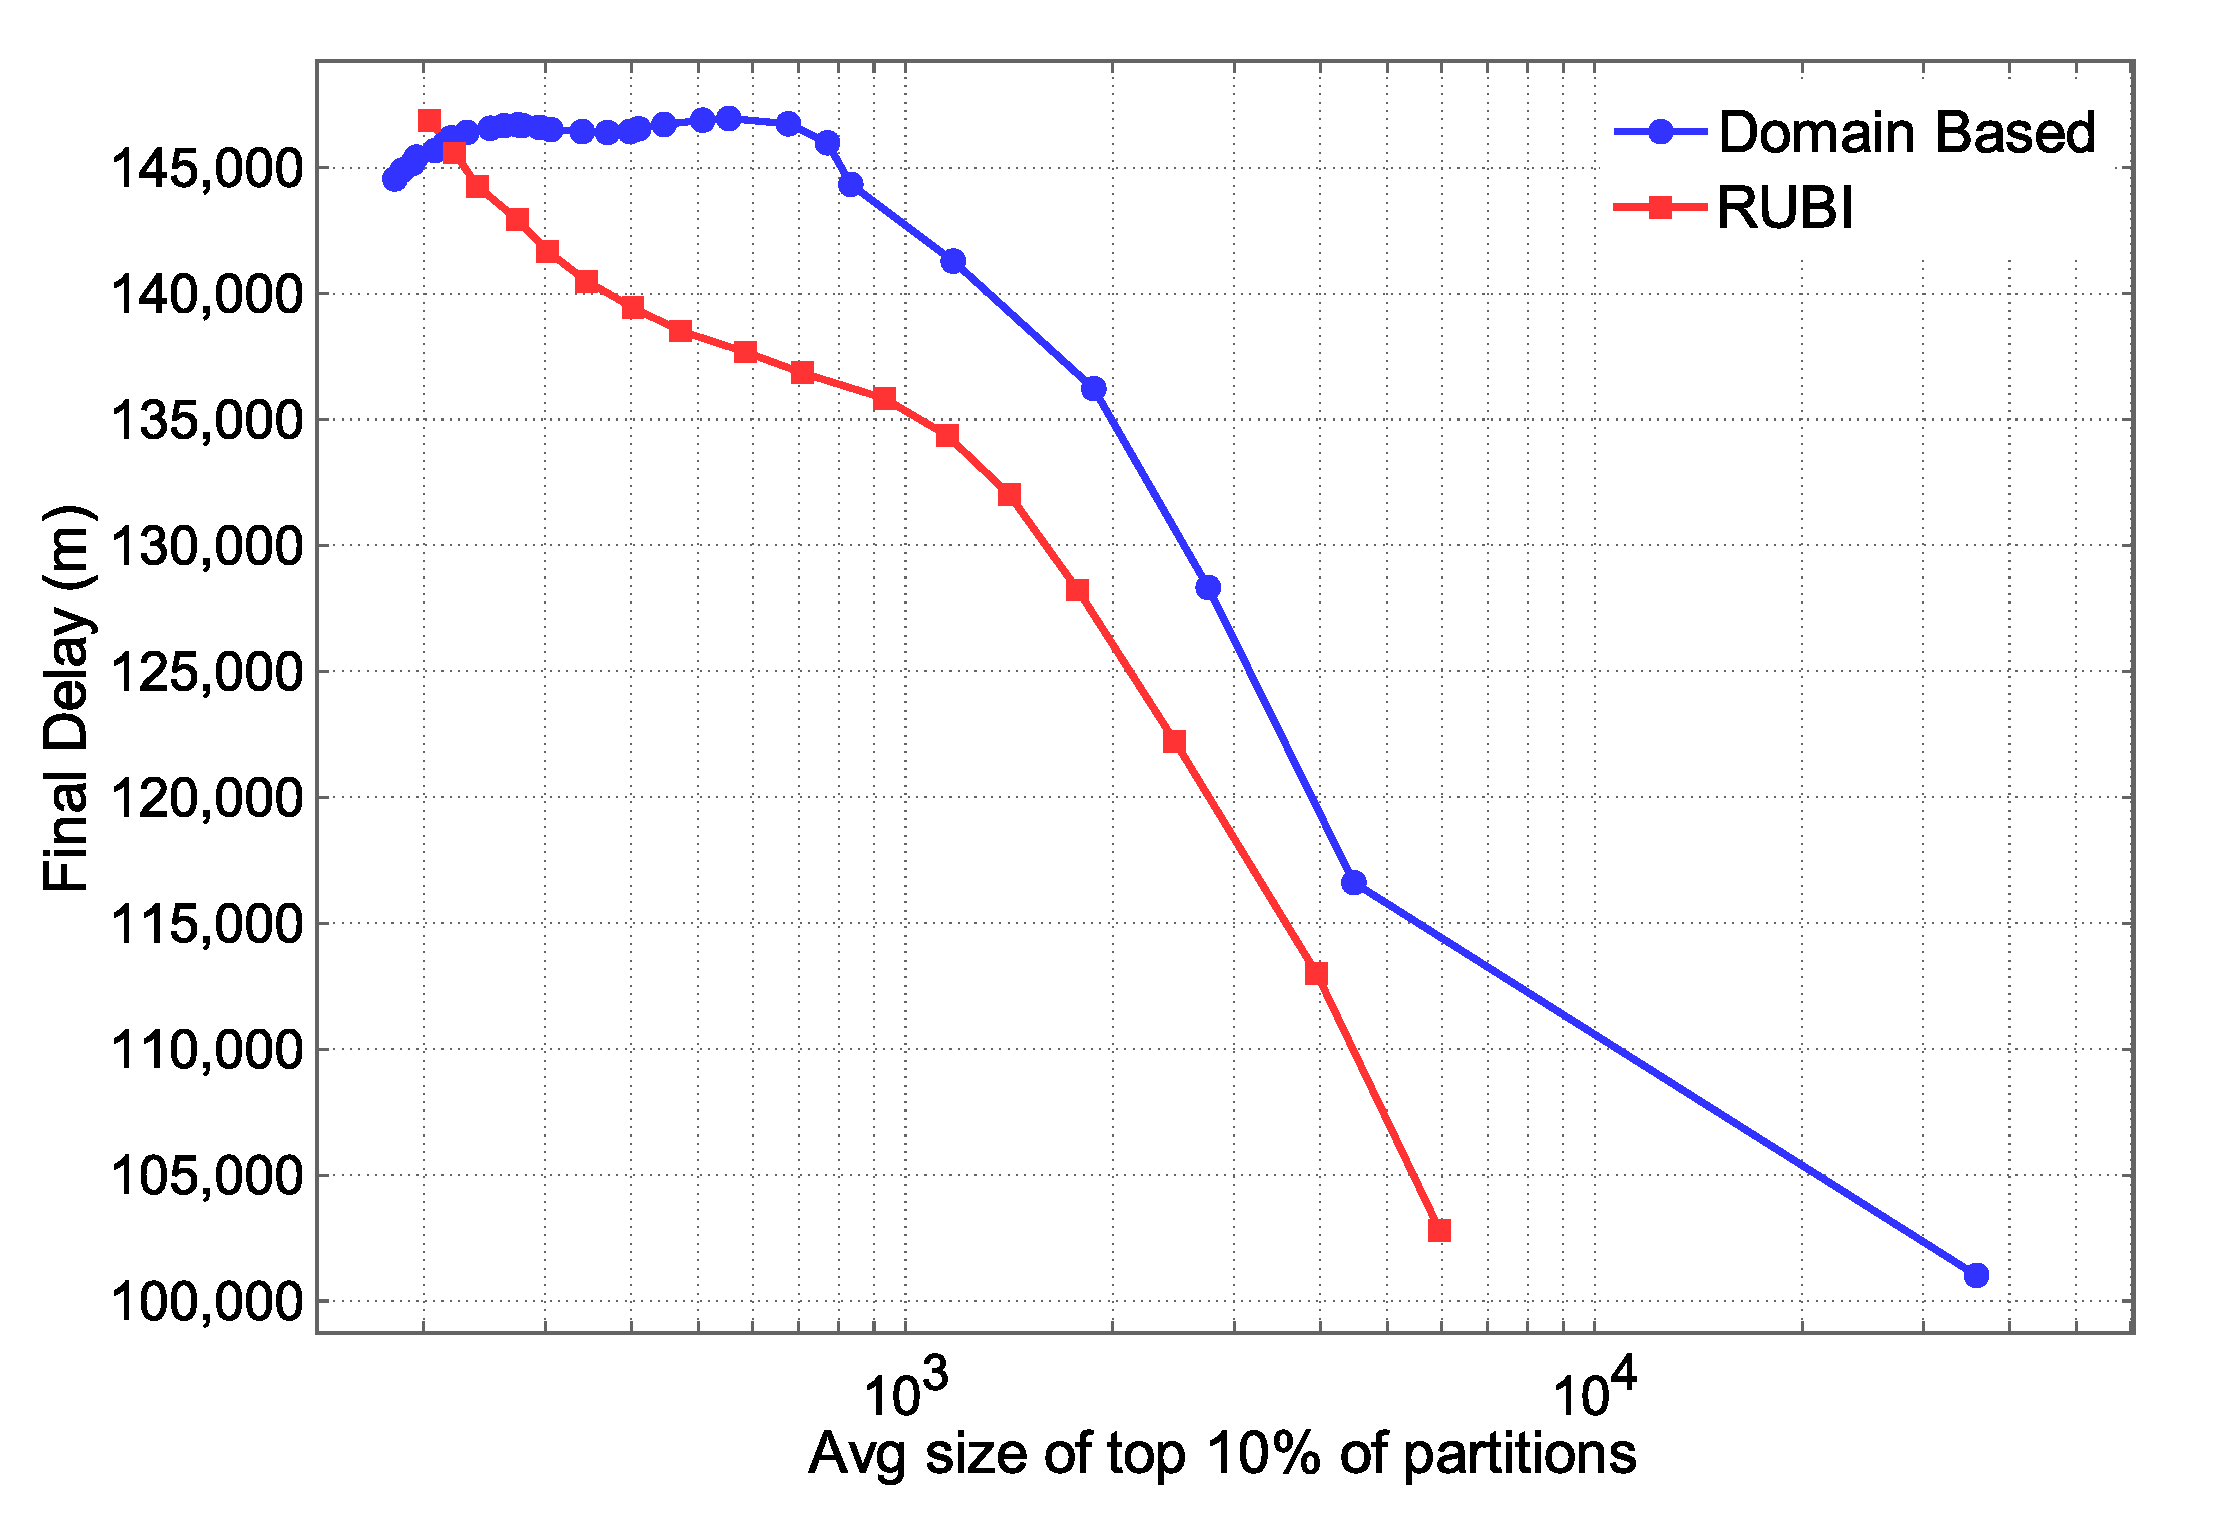
\includegraphics[width=1.0\columnwidth]{ATFMPPerformancevsAvgSize}
%\caption{When comparing individual partition size averages to performance, RUBI partitions perform much better than domain specific %partitions with respect to average partition size and final performance.}
%\label{ATFMPPerformancevsAvgSize}
%\end{figure}
\section{Comparison Between RUBI and Domain-Based Partitioning}
\label{sec:Comparison}
%To understand how much overlap partitions had with each other, we analyzed the similarity each partition had with itself, and the average similarity each partition had with other partitions. Similarity was defined as the similarity metric used in Section \ref{sec:Domain-Based}, the number of similar sectors between agents.

%\begin{figure}
%\centering
%\includegraphics[width=.75\columnwidth]{Self-SimOldvsSelf-SimNew}
%\caption{Partitions formed with RUBI had higher self-similarity than those made using domain-based partitioning. This leads to %higher-quality learning with respect to each partition.}
%\label{Self-SimOldvsSelf-SimNew}
%\end{figure}

\begin{figure}
\centering
\includegraphics[width=.75\columnwidth]{FinalOldvsFinalNew}
\caption{The final performance of RUBI partitions compared to domain-based partitions. In highly-partitioned cases, domain-based partitions perform better than RUBI, with RUBI performing better with a smaller number of partitions.}
\label{FinalOldvsFinalNew}
\end{figure}

\begin{figure}
\centering
\includegraphics[width=.75\columnwidth]{OldvsNewAvgSize}
\caption{In highly-partitioned cases, domain-based partitioning has a larger average size of the top 5\% of partitions, leading to a higher initial performance (Figure 6). With a smaller number of partitions, RUBI partitioning had a larger size of partitions. Note that when all partitions are reward independent, domain-based partitioning had only a few large partitions. RUBI partitioning on the other hand included a much smaller average size, and many more partitions. Smaller and more numerous partitions lead to faster simulations (Section \ref{sec:Complexity}).}
\label{OldvsNewAvgSize}
\end{figure}

\begin{figure}
\centering
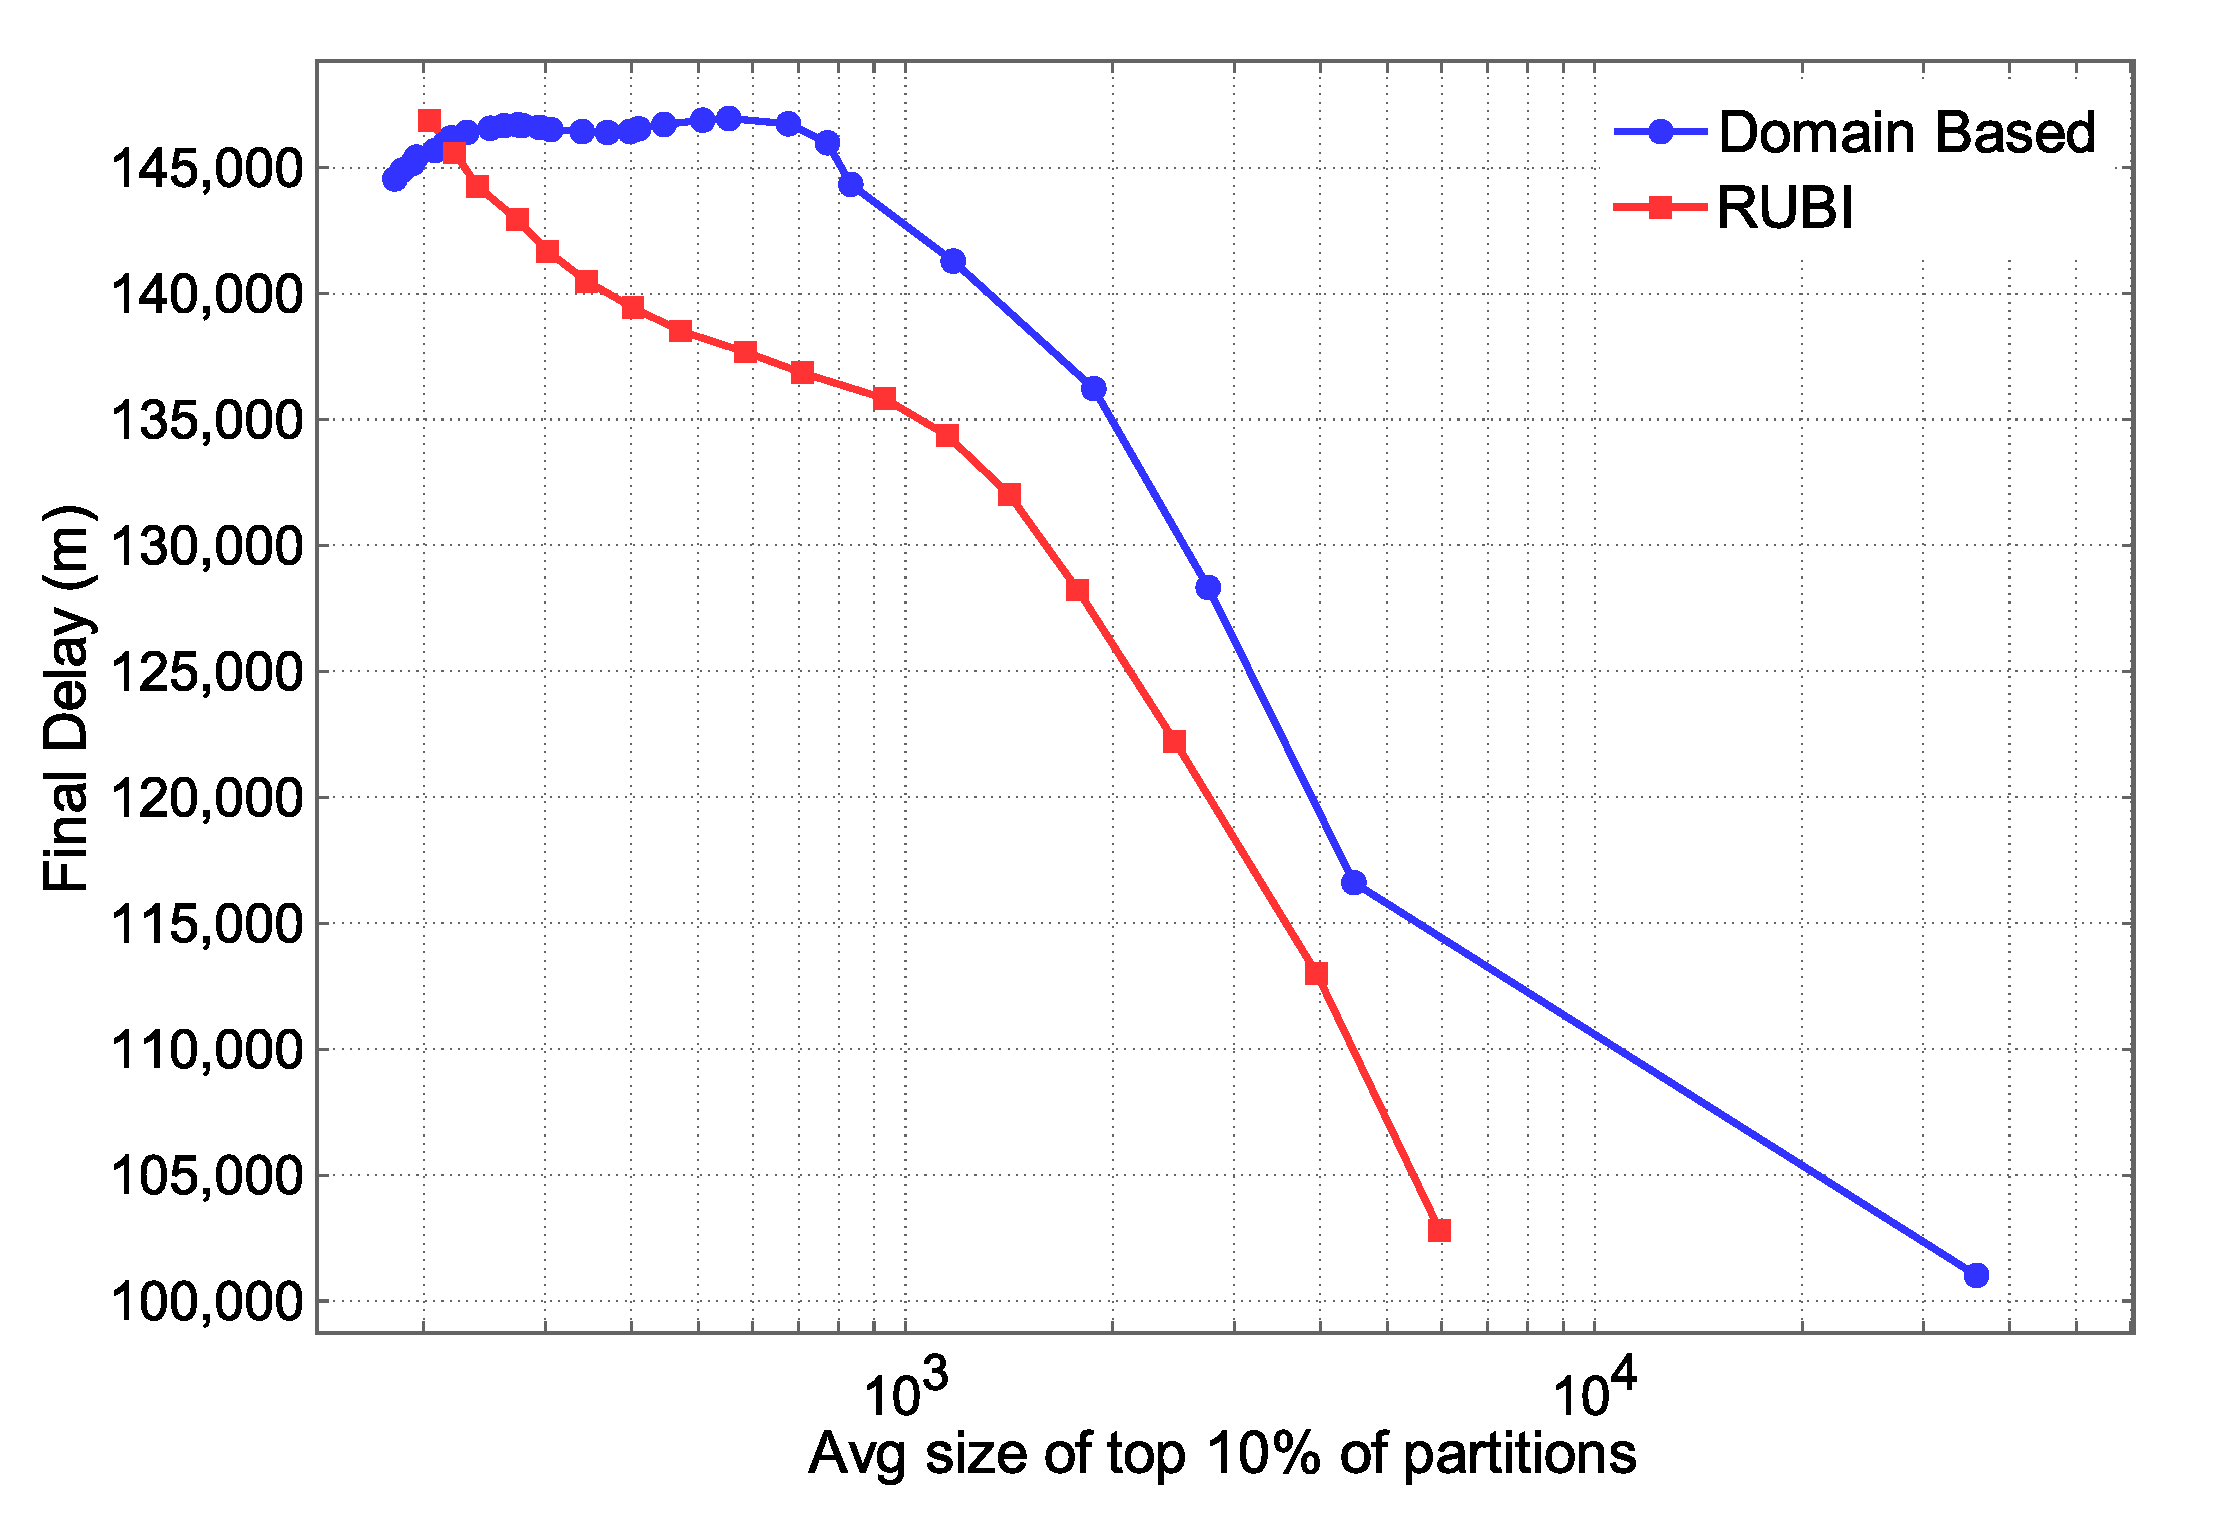
\includegraphics[width=.75\columnwidth]{ATFMPPerformancevsAvgSize}
\caption{When comparing individual partition size averages to performance, RUBI partitions perform much better than domain specific partitions with respect to average partition size and final performance.}
\label{ATFMPPerformancevsAvgSize}
\end{figure}

%To understand how much overlap partitions had with each other, we analyzed the similarity each partition had with itself, and the average similarity each partition had with other partitions. Similarity was defined as the similarity metric used in Section \ref{sec:Domain-Based}, the number of similar sectors between agents.

%In this section, we find the percentage of sectors that are similar between aircraft in a partition (self-similarity). In a purely reward independent partition, the self-similarity is 1. As the amount of self similarity increases, the computation time increases exponentially, and the benefits of partitioning decreases, as described in Section \ref{sec:Complexity} and shown in the Section \ref{sec:Domain-Based}. 

%Partitioning with RUBI developed better similarity scores than domain-based partitioning (Figure \ref{Self-SimOldvsSelf-SimNew}). By partitioning using congestion, rather than similar sectors, the similarity metric was able to represent both similar sectors as well as sector congestion. For example, two aircraft have the same flight plan, excluding their congested arrival and departure location. These aircraft would be partitioned together when using only similar sector domain knowledge. With RUBI, those aircraft would be partitioned together with aircraft that cause them congestion. By partitioning using the impact one agent had on another agents reward, we are able to formulate higher quality partitions, without the overhead of developing similarity metrics or learning domain knowledge.

Partitioning using RUBI converged to a reward independent partitioning that included many more partitions than domain-based partitioning. The converged domain-based partitioning included 3 partitions, while partitioning with RUBI included 61 partitions. This is due to using reward-based impact as a clustering metric, as mentioned in Section \ref{sec:Complexity}. Two actions may greatly affect each other during simulation, but their reward-based impact on each other might still be zero. This is important to keep in mind during partition analysis. For example, if two agents go through the same sectors, but neither agent causes another agent more or less congestion, then the difference in local reward will be zero, even though those aircraft affect each other. This leads to more partitions, and therefore faster simulations.

When comparing final performance, a direct comparison of performance is informative, but not entirely adequate. This is because partitions are not evenly distributed, which causes extremely large bias when comparing final performance to number of partitions. Figure \ref{FinalOldvsFinalNew} shows that domain-based partitioning initially out performs RUBI, but RUBI began out performing domain-based partitioning with a smaller number of partitions. When analyzing the reason behind this, we found that partitions are not evenly distributed (Figure \ref{OldvsNewAvgSize}). Initially, domain-based partitioning have large partitions compared to RUBI partitioning. This is due to the accumulation of similar sectors in domain-based partitioning. In domain-based partitioning, all of the planes with high overlap are initially merged together, giving domain-based partitioning initially larger partitions. Since this is a highly coupled domain, this also leads to one partition becoming much larger than others.

RUBI, which partitions based on the reward of congestion, initially merged together partitions whose reward highly impacted each other. This creates more evenly distributed partitions, a desired quality during complexity analysis (Section \ref{sec:Complexity}). Even though this leads to a better final performance, it causes initially worse performance (Figure \ref{FinalOldvsFinalNew}). It is useful to note that in these cases where domain-based partitioning performed better, the performance was only 5\% better than the greedy scheduler.

This results in us comparing final performance to the average size of the largest 5\% of partitions. This gives a comparison of how well a partitioning performs with respect to the size of its partitions, rather than the number. Figure \ref{ATFMPPerformancevsAvgSize} shows that initially in domain-based partitioning, learning performance does not increase with respect to the average size of the partitions. RUBI on the other hand creates a partitioning with constantly increasing performance. 

As also shown in Figure \ref{FinalOldvsFinalNew}, with more partitions domain-based partitioning performs better than RUBI. In this case domain-based partitioning remains static as the average size of partitions decreases, while the performance of RUBI increases. Although these partitions are too large to be of use during learning, it is interesting to note that in this case, domain-based partitioning performs better than RUBI. The reasoning behind this is similar to the reasoning behind Figure \ref{FinalOldvsFinalNew}, with a greater number of partitions it is more informative for agents to be partitioned together using strict sector similarity counts than using reward impacts. With fewer partitions though, reward impacts are much more useful as a partitioning metric. RUBI partitions perform better and lead to faster simulation times.

%then $c$ becomes larger and $c_n$ becomes smaller, meaning less agents per partition and faster computation time.

\section{Conclusion}

Current approaches in multiagent learning with partitioning create well-performing agents. However, these approaches do not scale to large multiagent domains \cite{Junges:2008:EPD:1402298.1402308,Modi:2005:AAD:1120120.1120127, Zhang:2010:SCD:1838206.1838304}, require expert domain knowledge to initially create the partitions \cite{Curran:2013:AHC:2484920.2485183,tumer-holmesparker_ala12,Proper:2012:MDR:2343896.2344025}, or use computationally expensive online modeling to approximate reward shaping \cite{Proper:2012:MDR:2343896.2344025}. This paper introduced RUBI, a general partitioning algorithm that computes reward-based impacts to perform agent partitioning, removing the need for prior knowledge of the system. Additionally, by removing all knowledge about the domain and instead partitioning based on reward, RUBI can be used to discover non-trivial indirect interactions encoded in a reward signal. Since RUBI uses only a reward signal to compute impacts, it will theoretically work in any domain where partitioning is useful and you have access to the reward signals.

%One of the key strengths of RUBI is its simplicity and generality combined with computing highly informative similarity scores. It needs no prior knowledge about the domain to perform partitioning, but instead simply needs a localized reward from each agent to build the similarity matrix. This localized reward can be easily obtained from the system-level reward or utility already developed for the learning approach. This makes RUBI highly generic and can be applied to any multiagent domain. It can treat the multiagent system as a black box, giving it random actions and receiving rewards. 

RUBI is likely to build more partitions without loss of performance. This leads to faster computation time due to fewer agents per partition. Since RUBI uses a localized reward as partitioning data, any effect one agent has on another agent will be encoded in this reward. For example, if an agent $a$ is removed from the system, and agent $b$'s reward changes, it means that agent $a$ affects agent $b$ in a direct or indirect way. In addition, if the congestion of each plane remains the same non-zero value, the actions do not affect the reward, therefore the agents are not partitioned. These indirect effects can be captured by RUBI and used as additional information when partitioning, leading to higher quality partitions in domains with complex interactions.

Lastly, RUBI was able to find an effective partitioning for 35,000 agents in the ATFMP in 2 hours. This is a pre-processing technique and is not included in the learning speed. RUBI was able to reduce the amount of computation in the ATFMP by hundreds of hours compared to the greedy scheduler, and therefore the additional computation is negligible. 

In this work, we showed that partitioning with RUBI accurately encapsulated the amount of coupling between agents, leading to a higher self-similarity metric over the domain-based partitioning, leading to faster simulation computation times. Learning using partitions developed with RUBI also found a 37\% increase in performance over the greedy solution with a 26x reduction in time complexity per learning step compared to the 23x reduction using domain-based partitioning. RUBI-based partitioning is able to achieve the same performance 15\% faster without a domain-specific similarity metric. RUBI's ability to calculate a larger number of smaller sized reward-independent partitions led to this reduction in simulation cost.

Future work in RUBI would involve performing a formal analysis of the relation between the number of iterations of RUBI and partition performance. Additionally, approximating the impact score of each agent, rather than using an accumulation, has the potential of being informative when performing an analysis of a system. %Lastly, performing distributed clustering would be an important, yet simple extension to this work.
\begin{acknowledgements}
This work was partially supported by the National Science Foundation under Grant No. CNS-0931591.
\end{acknowledgements}
\label{sec:CONCLUSION}


\bibliographystyle{spbasic}
\bibliography{thesis}

\end{document}
